

\begin{tikzpicture}[line width=1.9mm]
\node[draw,scale=4,fill=yellow!80!black]{Cap.3 \  O Campo Elétrico};
\end{tikzpicture} 


\begin{tikzpicture}[line width=1.1mm]
\node[draw,scale=2,fill=blue!20!red]{Ex.1};
\end{tikzpicture} 

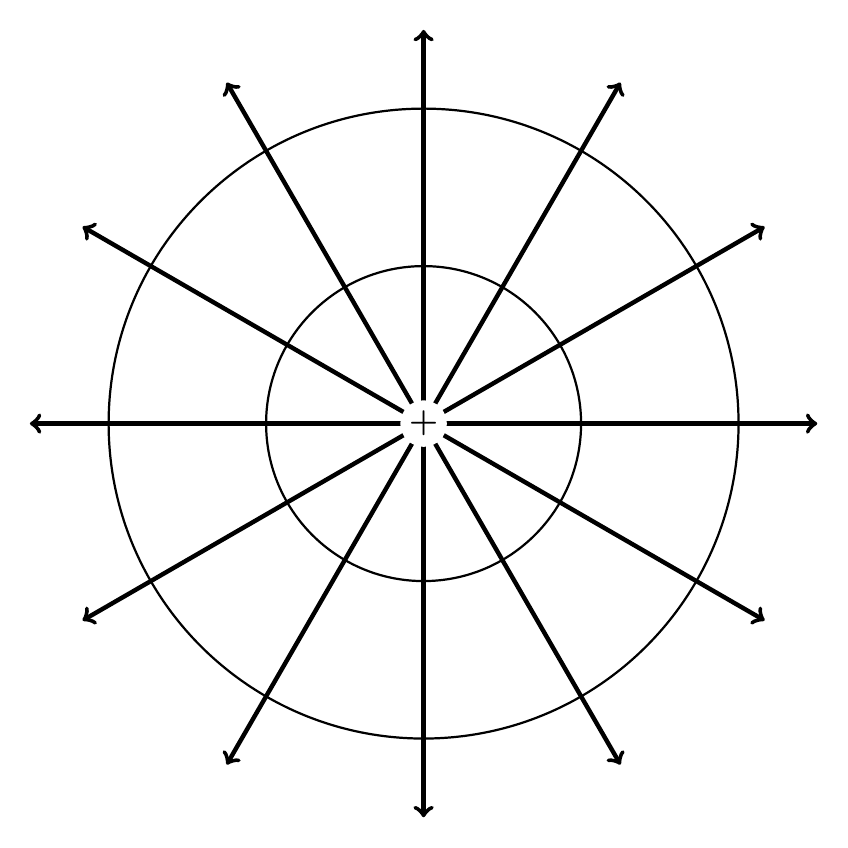
\begin{tikzpicture}[line width=1.9mm]
%linhas de campo
  \draw[ultra thick,<->] (-5,0) -- ( 5,0);
  \draw[ultra thick,<->] (-4.33,-2.5) -- (4.33,2.5);
  \draw[ultra thick,<->] (-2.5,-4.33) -- (2.5,4.33);
  \draw[ultra thick,<->] (0,-5) -- (0,5);
  \draw[ultra thick,<->] (2.5,-4.33) -- (-2.5,4.33);
  \draw[ultra thick,<->] (4.33,-2.5) -- (-4.33,2.5);
%superfícies equipotenciais
   \filldraw [white] (0,0) circle (0.2);
   \draw[thick] (2,0) arc (0:360:2);
   \draw[thick] (4,0) arc (0:360:4);
%rótulos
  \filldraw[] (0,0) node[font=\fontsize{12pt}{12pt}\selectfont,] {$\textbf{+}$};
\end{tikzpicture} 

%linhas soverdouro
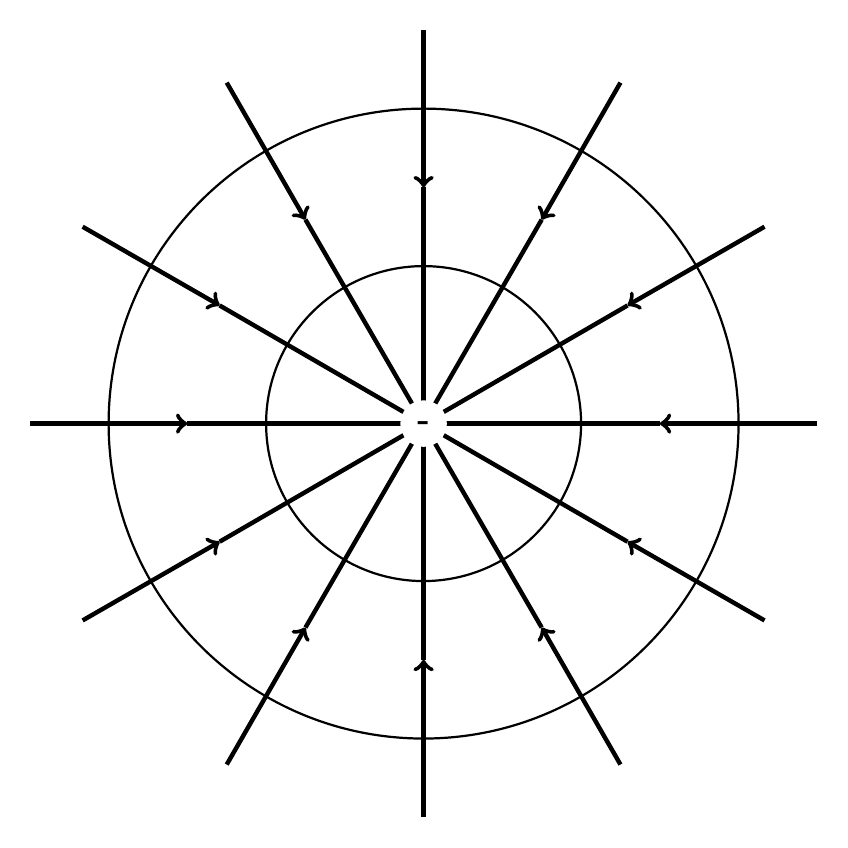
\begin{tikzpicture}[line width=1.9mm]
%linhas de campo
  \draw[ultra thick,<-] (3,0) -- (5,0);
  \draw[ultra thick] (3,0) -- ( 0,0);
  \draw[ultra thick,<-] (2.59,1.5) -- (4.33,2.5);
  \draw[ultra thick] (2.59,1.5) -- (0,0);
  \draw[ultra thick,<-] (1.5,2.59) -- (2.5,4.33);
  \draw[ultra thick] (1.5,2.59) -- (0,0);
  \draw[ultra thick,<-] (0,3) -- (0,5);
  \draw[ultra thick] (0,3) -- (0,0);
  
  \draw[ultra thick,<-] (-2.59,1.5) -- (-4.33,2.5);
  \draw[ultra thick] (-2.59,1.5) -- (0,0);
  \draw[ultra thick,<-] (-1.5,2.59) -- (-2.5,4.33);
  \draw[ultra thick] (-1.5,2.59) -- (0,0);
  
  \draw[ultra thick,<-] (-3,0) -- (-5,0);
  \draw[ultra thick] (-3,0) -- (0,0);
  \draw[ultra thick,<-] (-2.59,-1.5) -- (-4.33,-2.5);
  \draw[ultra thick] (-2.59,-1.5) -- (0,0);
  \draw[ultra thick,<-] (-1.5,-2.59) -- (-2.5,-4.33);
  \draw[ultra thick] (-1.5,-2.59) -- (0,0);
  \draw[ultra thick,<-] (0,-3) -- (0,-5);
  \draw[ultra thick] (0,-3) -- (0,0);
  
  \draw[ultra thick,<-] (2.59,-1.5) -- (4.33,-2.5);
  \draw[ultra thick] (2.59,-1.5) -- (0,0);
  \draw[ultra thick,<-] (1.5,-2.59) -- (2.5,-4.33);
  \draw[ultra thick] (1.5,-2.59) -- (0,0);


%superfícies equipotenciais
   \filldraw [white] (0,0) circle (0.2);
   \draw[thick] (2,0) arc (0:360:2);
   \draw[thick] (4,0) arc (0:360:4);
%rótulos
  \filldraw[] (0,0) node[font=\fontsize{12pt}{12pt}\selectfont,] {$\textbf{-}$};
\end{tikzpicture} 


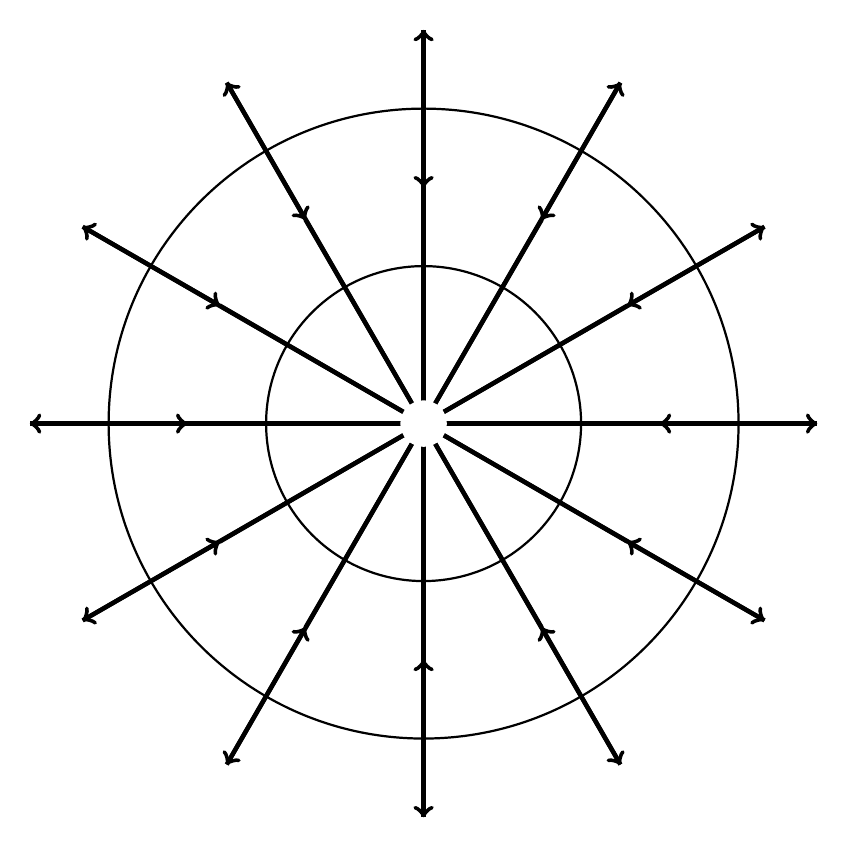
\begin{tikzpicture}[line width=1.9mm]
%linhas de campo fonte
  \draw[ultra thick,<->] (-5,0) -- ( 5,0);
  \draw[ultra thick,<->] (-4.33,-2.5) -- (4.33,2.5);
  \draw[ultra thick,<->] (-2.5,-4.33) -- (2.5,4.33);
  \draw[ultra thick,<->] (0,-5) -- (0,5);
  \draw[ultra thick,<->] (2.5,-4.33) -- (-2.5,4.33);
  \draw[ultra thick,<->] (4.33,-2.5) -- (-4.33,2.5);
%linhas de campo sorvedouro
  \draw[ultra thick,<-] (3,0) -- (5,0);
  \draw[ultra thick] (3,0) -- ( 0,0);
  \draw[ultra thick,<-] (2.59,1.5) -- (4.33,2.5);
  \draw[ultra thick] (2.59,1.5) -- (0,0);
  \draw[ultra thick,<-] (1.5,2.59) -- (2.5,4.33);
  \draw[ultra thick] (1.5,2.59) -- (0,0);
  \draw[ultra thick,<-] (0,3) -- (0,5);
  \draw[ultra thick] (0,3) -- (0,0);
  
  \draw[ultra thick,<-] (-2.59,1.5) -- (-4.33,2.5);
  \draw[ultra thick] (-2.59,1.5) -- (0,0);
  \draw[ultra thick,<-] (-1.5,2.59) -- (-2.5,4.33);
  \draw[ultra thick] (-1.5,2.59) -- (0,0);
  
  \draw[ultra thick,<-] (-3,0) -- (-5,0);
  \draw[ultra thick] (-3,0) -- (0,0);
  \draw[ultra thick,<-] (-2.59,-1.5) -- (-4.33,-2.5);
  \draw[ultra thick] (-2.59,-1.5) -- (0,0);
  \draw[ultra thick,<-] (-1.5,-2.59) -- (-2.5,-4.33);
  \draw[ultra thick] (-1.5,-2.59) -- (0,0);
  \draw[ultra thick,<-] (0,-3) -- (0,-5);
  \draw[ultra thick] (0,-3) -- (0,0);
  
  \draw[ultra thick,<-] (2.59,-1.5) -- (4.33,-2.5);
  \draw[ultra thick] (2.59,-1.5) -- (0,0);
  \draw[ultra thick,<-] (1.5,-2.59) -- (2.5,-4.33);
  \draw[ultra thick] (1.5,-2.59) -- (0,0);


%superfícies equipotenciais
   \filldraw [white] (0,0) circle (0.2);
   \draw[thick] (2,0) arc (0:360:2);
   \draw[thick] (4,0) arc (0:360:4);
%rótulos
  \filldraw[] (0,0) node[font=\fontsize{12pt}{12pt}\selectfont,] {$\textbf{}$};
\end{tikzpicture} 


\begin{tikzpicture}[line width=1.1mm]
\node[draw,scale=2,fill=blue!20!red]{Ex.2};
\end{tikzpicture}

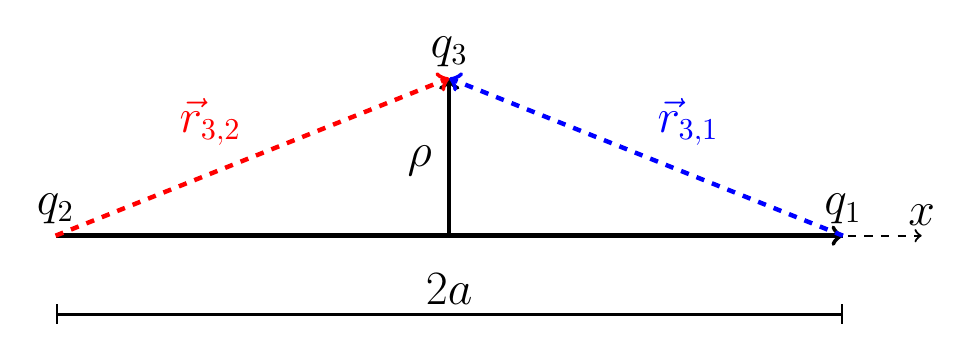
\begin{tikzpicture}[line width=0.7mm]
  %eixos
  \draw[dashed,thick,->] (0,0) -- ( 6,0) node[font=\fontsize{16pt}{16pt}\selectfont,anchor=south]{$x$};
  
  \coordinate (v1) at (-5,0);
  \coordinate (v3) at (5,0);
  \coordinate (v4) at (-5,-1);
  \coordinate (v5) at (5,-1);
  % add coordinate at the extension of the line from v1 to v2
 
  %o primeiro termo entre colchetes acima, seleciona o tamanho da fonte
  %já o último termo posiciona a figura
  \draw  (v3) -- (v1)node[font=\fontsize{16pt}{16pt}\selectfont,above] {$q_{2}$};
  %rótulo das alturas,lados...
  \put(-15,25){font=\fontsize{16pt}{16pt}\selectfont$\rho$};
  \draw[thick,|-|]  (v4) -- node[font=\fontsize{16pt}{16pt}\selectfont,above] {$2a$}(v5);
  \draw[,ultra thick,->] (0,0) -- ( 0,2)node[font=\fontsize{16pt}{16pt}\selectfont,above] {$q_{3}$};
  \draw[,ultra thick,->] (0,0) --(v3)node[font=\fontsize{16pt}{16pt}\selectfont,above] {$q_{1}$};
  \draw[dashed,blue,ultra thick,->] (v3) --node[font=\fontsize{16pt}{16pt}\selectfont,above right] {$\vec{r}_{3,1}$} (0,2);
  \draw[dashed,red,ultra thick,->] (v1) --node[font=\fontsize{16pt}{16pt}\selectfont,above left] {$\vec{r}_{3,2}$} (0,2);
\end{tikzpicture}



\begin{tikzpicture}[line width=1.1mm]
\node[draw,scale=2,fill=blue!20!red]{Ex.3};
\end{tikzpicture} 

\tdplotsetmaincoords{60}{120}
\begin{tikzpicture}[tdplot_main_coords]

  % axes
  \draw[dashed,thick,->] (-7,0,0) -- ( 7,0,0) node[anchor=west]{$x$};
  \draw[dashed,thick,->] (0,-7,0) -- ( 0,7,0) node[anchor=west]{$y$};
  \draw[dashed,thick,->] (0,0,0) -- ( 0,0,5) node[anchor=west]{$z$};

  % vetor 1
  \pgfmathsetmacro{\ax}{6}
  \pgfmathsetmacro{\ay}{-6}
  \pgfmathsetmacro{\az}{0}
  \draw[very thick,->,red] (0,0,0) --node[above]{$\rho$}node[below]{\fontsize{16pt}{16pt}\selectfont$\vec{r'}$} (1.5,-2.6,\az);
  % vetor 2
  \draw[very thick,->,red] (0,0,\az) --node[left]{D}node[right]{\fontsize{16pt}{16pt}\selectfont$\vec{r}$} (0,0,4);

   % dashed plano
  \draw[dashed,gray] (-\ax,\ay,0) -- (\ax,\ay,0);
  \draw[dashed,gray] (\ax,-\ay,0) -- (\ax,\ay,0);
  \draw[dashed,gray] (-\ax,-\ay,0) -- (-\ax,\ay,0);
  \draw[dashed,gray] (\ax,-\ay,0) -- (-\ax,-\ay,0);
  
  % cargas
  \put(50,-50,0){font=\fontsize{16pt}{16pt}\selectfont$\sigma$};
  
  % Superfície gaussiana
  \draw[thick,orange] (3,0,0) arc (0:360:3);
  \draw[thick,orange] (3,0,4) arc (0:360:3);
  \draw[thick,orange,-] (1.5,-2.6,\az) -- (1.5,-2.6,4);
  \draw[thick,orange,-] (-1.5,2.6,\az) -- (-1.5,2.6,4);
\end{tikzpicture}


\begin{tikzpicture}[line width=1.1mm]
\node[draw,scale=2,fill=blue!20!red]{Ex.4};
\end{tikzpicture}

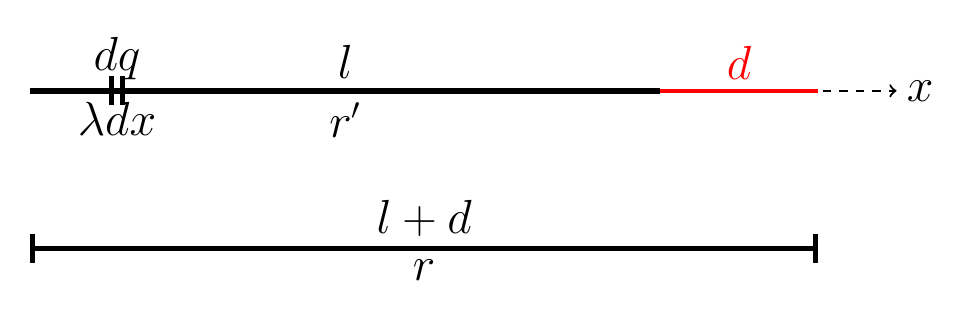
\begin{tikzpicture}[line width=0.7mm]
  %eixos
  \draw[dashed,thick,->] (0,0) -- ( 6,0) node[font=\fontsize{16pt}{16pt}\selectfont,right]{$x$};
  %barra de cima(fio)
  \coordinate (v1) at (-5,0);
  \coordinate (v3) at (3,0);
  \coordinate (v6) at (-4,0);
  \coordinate (v7) at (-3.8,0);
  \coordinate (v8) at (5,0);
  
  \draw  (v3) -- node[font=\fontsize{16pt}{16pt}\selectfont,below] {$r'$}node[font=\fontsize{16pt}{16pt}\selectfont,above] {$l$}(v1);
  \draw[red,ultra thick,-]  (v3) -- node[font=\fontsize{16pt}{16pt}\selectfont,above]{$d$}(v8);

  \draw[ultra thick,|-|]  (v6) -- node[font=\fontsize{16pt}{16pt}\selectfont,above]{$dq$}node[font=\fontsize{16pt}{16pt}\selectfont,below] {$\lambda dx$}(v7);
  
  %barra de baixo(escala)
  \coordinate (v4) at (-5,-2);
  \coordinate (v5) at (5,-2);
  
  \draw[ultra thick,|-|]  (v4) -- node[font=\fontsize{16pt}{16pt}\selectfont,above] {$l+d$}node[font=\fontsize{16pt}{16pt}\selectfont,below] {$r$}(v5);
  
\end{tikzpicture}


\begin{tikzpicture}[line width=1.1mm]
\node[draw,scale=2,fill=blue!20!red]{Ex.5};
\end{tikzpicture}

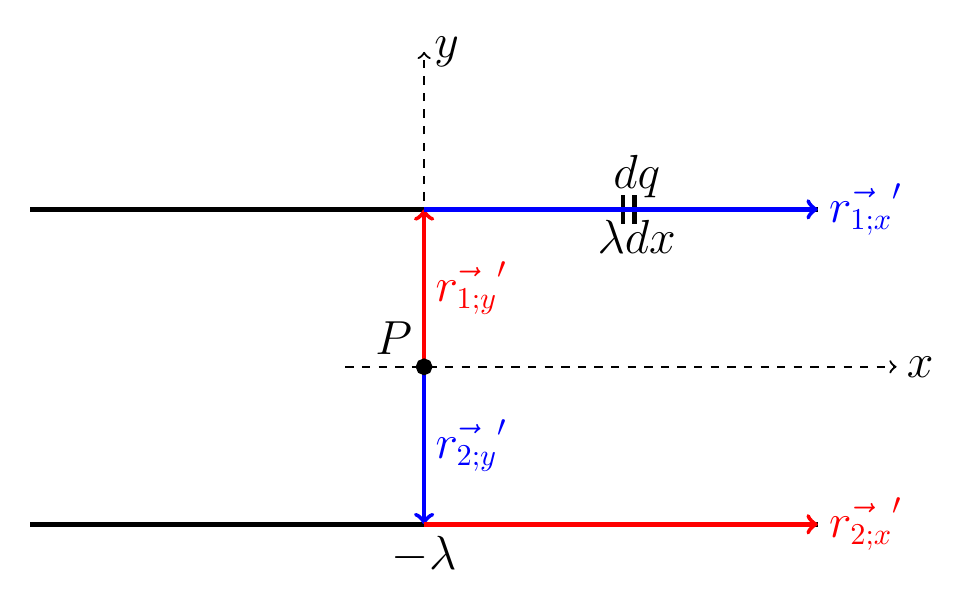
\begin{tikzpicture}[line width=0.7mm]
  %eixos
  \draw[dashed,thick,->] (-1,-2) -- ( 6,-2) node[font=\fontsize{16pt}{16pt}\selectfont,right]{$x$};
  \draw[dashed,thick,->] (0,-2) -- ( 0,2) node[font=\fontsize{16pt}{16pt}\selectfont,right]{$y$};
  %barra de cima(fio)
  \coordinate (v1) at (-5,0);
  \coordinate (v3) at (5,0);
  \coordinate (v6) at (-4,0);
  \coordinate (v7) at (2.7,0);
  \coordinate (v2) at (2.5,0);
  
  \draw (v3) -- (v1);

  \draw[ultra thick,|-|]  (v2) -- (v7)node[font=\fontsize{16pt}{16pt}\selectfont,above]{$dq$}node[font=\fontsize{16pt}{16pt}\selectfont,below] {$\lambda dx$};
  
  %barra de baixo
  \coordinate (v4) at (-5,-4);
  \coordinate (v5) at (5,-4);
  
  \draw (v4) -- node[font=\fontsize{16pt}{16pt}\selectfont,below] {$-\lambda$}(v5);
  
  %vetores
  \coordinate (v8) at (0,-2);
  \coordinate (v9) at (0,0);
  \coordinate (v10) at (5,0);
  
  \coordinate (v11) at (0,-2);
  \coordinate (v12) at (0,-4);
  \coordinate (v13) at (5,-4);
  
  \draw[red,ultra thick,->] (v8) -- node[font=\fontsize{16pt}{16pt}\selectfont,right] {$\vec{r_{1;y}}'$}(0,0);
  \draw[blue,ultra thick,->] (v9) -- (v10)node[font=\fontsize{16pt}{16pt}\selectfont,right] {$\vec{r_{1;x}}'$};
  
  \draw[blue,ultra thick,->] (v11) -- node[font=\fontsize{16pt}{16pt}\selectfont,right] {$\vec{r_{2;y}}'$}(v12);
  \draw[red,ultra thick,->] (v12) -- (v13)node[font=\fontsize{16pt}{16pt}\selectfont,right] {$\vec{r_{2;x}}'$};
  
  %Ponto de observação
  \filldraw[black] (v11) circle (2pt) node[font=\fontsize{16pt}{16pt}\selectfont,above left] {$P$};
  
\end{tikzpicture}


\begin{tikzpicture}[line width=1.1mm]
\node[draw,scale=2,fill=blue!20!red]{Ex.6};
\end{tikzpicture} 

\tdplotsetmaincoords{60}{120}
\begin{tikzpicture}[tdplot_main_coords]

  % axes
  \draw[dashed,thick,->] (-7,0,0) -- ( 7,0,0) node[anchor=west]{$x$};
  \draw[dashed,thick,->] (0,-7,0) -- ( 0,7,0) node[anchor=west]{$y$};
  \draw[dashed,thick,->] (0,0,0) -- ( 0,0,5) node[anchor=west]{$z$};

  % vetor 1
  \pgfmathsetmacro{\ax}{6}
  \pgfmathsetmacro{\ay}{-6}
  \pgfmathsetmacro{\az}{0}
  \draw[very thick,->,red] (0,0,0) --node[anchor=south west ]{\fontsize{16pt}{16pt}\selectfont$\vec{r'}$} (\ax,-\ay,\az);
  % vetor 2
  \draw[very thick,->,brown] (0,0,\az) --node[left]{D}node[right]{\fontsize{16pt}{16pt}\selectfont$\vec{r}$} (0,0,4)node[right]{\fontsize{16pt}{16pt}\selectfont$\vec{P}$};
  % vetor 3
  \draw[very thick,->,blue] (0,0,0) --node[below]{\fontsize{16pt}{16pt}\selectfont$\vec{y}$} (0,-\ay,\az);
  \draw[very thick,->,blue] (0,-\ay,\az) --node[below]{\fontsize{16pt}{16pt}\selectfont$\vec{l}$} (\ax,-\ay,\az);

   % dashed plano
  \draw[dashed,gray] (-\ax,\ay,0) -- (\ax,\ay,0);
  \draw[dashed,gray] (\ax,-\ay,0) -- (\ax,\ay,0);
  \draw[dashed,gray] (-\ax,-\ay,0) -- (-\ax,\ay,0);
  \draw[dashed,gray] (\ax,-\ay,0) -- (-\ax,-\ay,0);
  
\end{tikzpicture}



